\documentclass[11pt, oneside]{article}
\usepackage[bottom=2.5cm,top=2.5cm]{geometry}
\geometry{a4paper}
\usepackage{graphicx}
\usepackage{amssymb}
\usepackage[utf8]{inputenc}
\usepackage[brazil]{babel}
\usepackage{color}
\usepackage{float}
\usepackage{hyperref}
\bibliographystyle{apalike}
\usepackage{indentfirst}

\title{Briefing Clima Espacial}
\date{25/04/2022}

\begin{document}
\maketitle 

 \section{Geomagnetism} 
 \subsection{Responsible: Livia Ribeiro Alves} 
 
\begin{figure}[H]
    
                        \centering
   
                             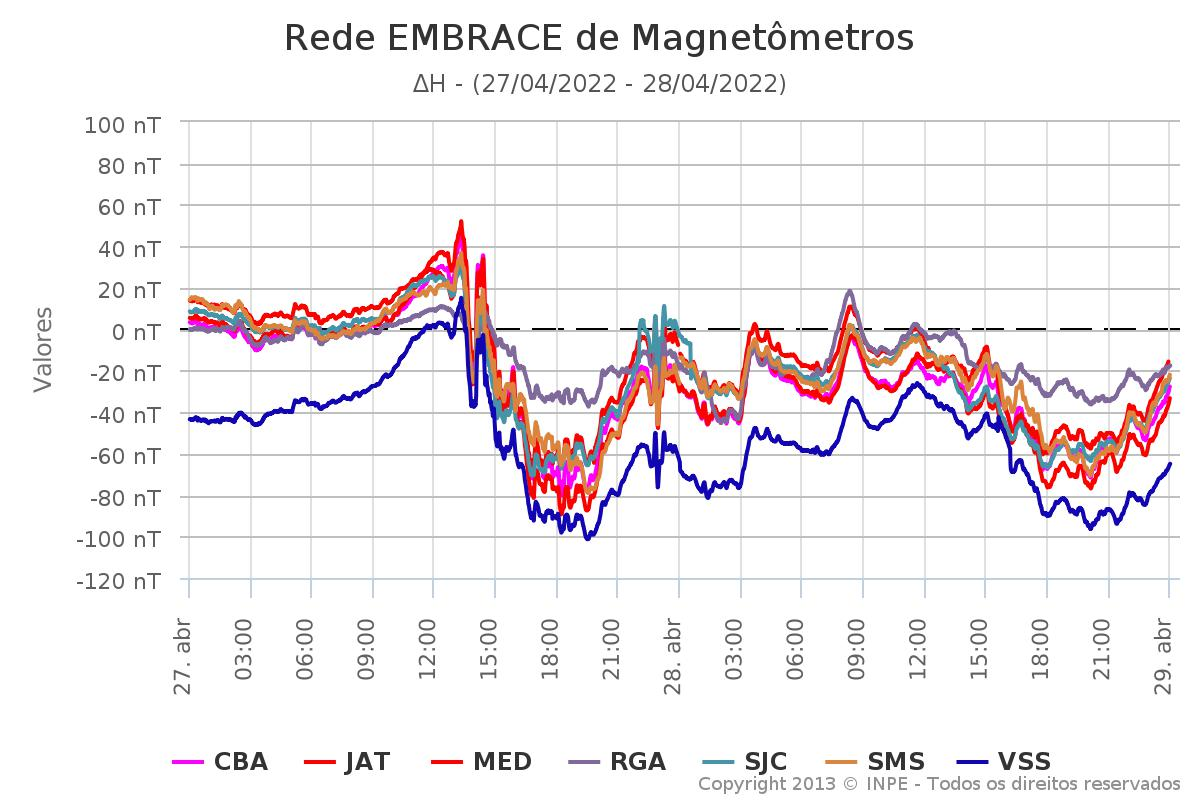
\includegraphics[width=14cm]{./figures/figureGeomag_0.png}

                        \end{figure}

                     \begin{figure}[H]
    
                        \centering
   
                             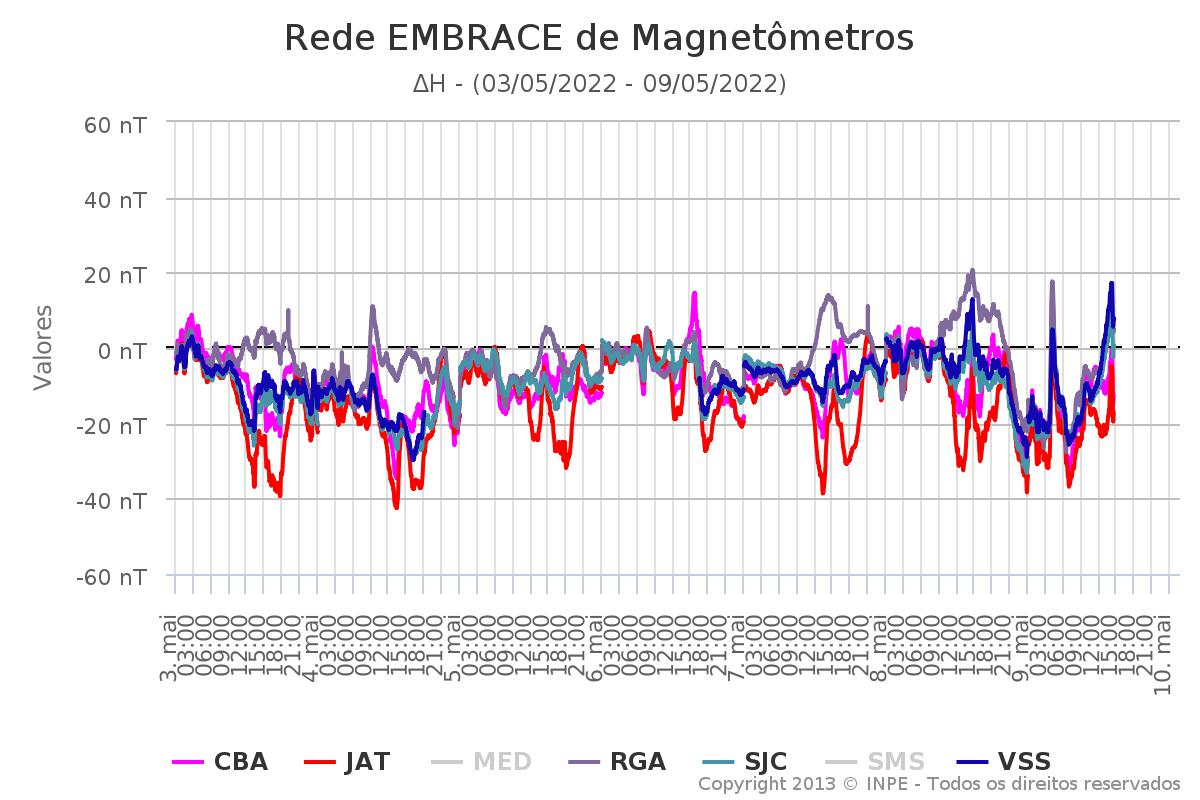
\includegraphics[width=14cm]{./figures/figureGeomag_1.png}

                        \end{figure}

                     \begin{figure}[H]
    
                        \centering
   
                             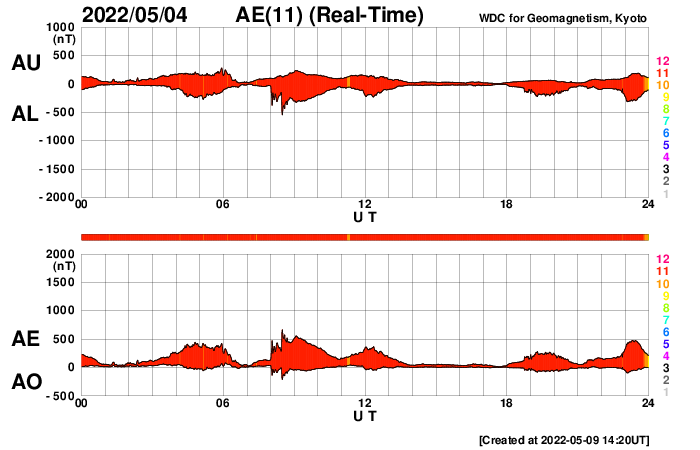
\includegraphics[width=14cm]{./figures/figureGeomag_2.png}

                        \end{figure}

                     \begin{figure}[H]
    
                        \centering
   
                             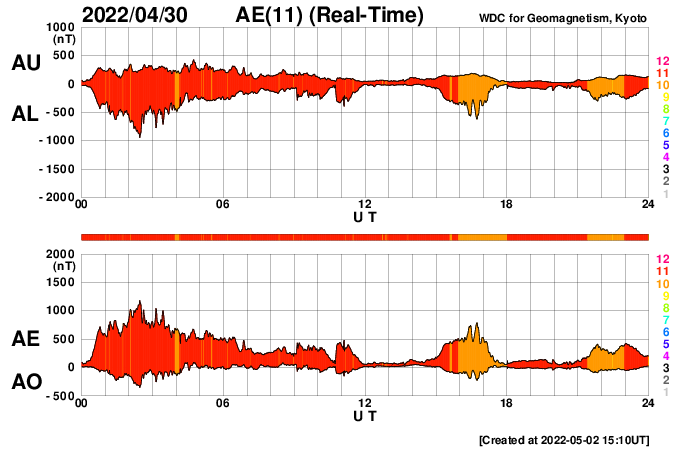
\includegraphics[width=14cm]{./figures/figureGeomag_3.png}

                        \end{figure}

                     \begin{figure}[H]
    
                        \centering
   
                             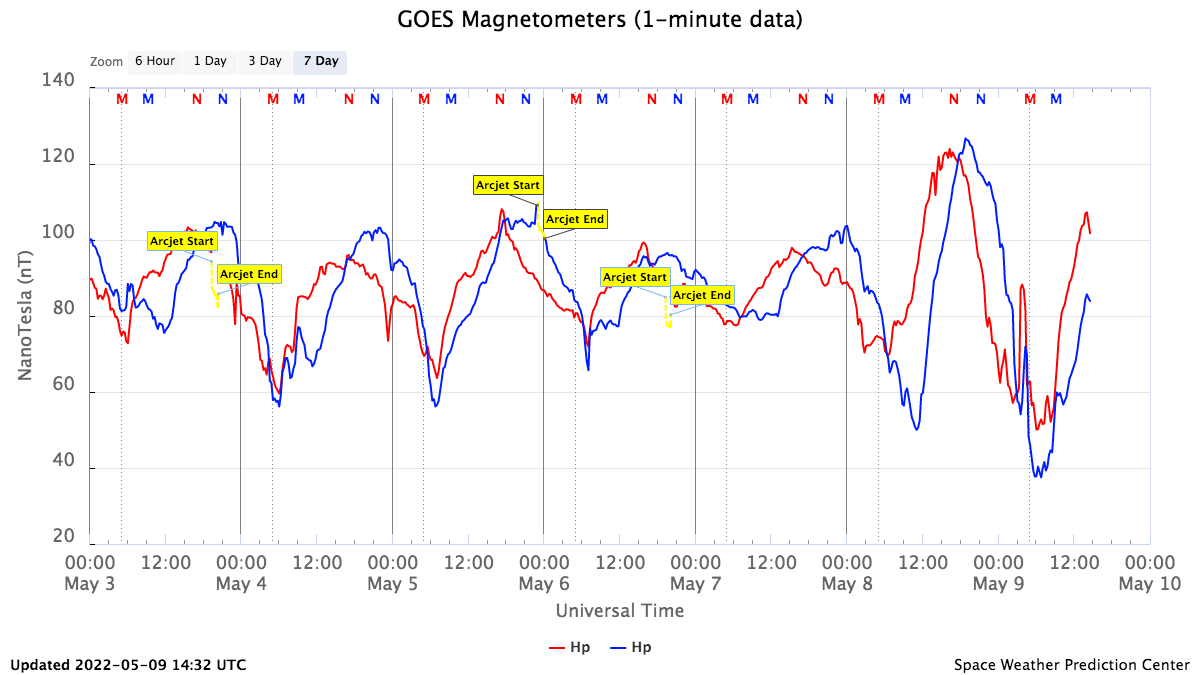
\includegraphics[width=14cm]{./figures/figureGeomag_4.png}

                        \end{figure}

                     \begin{figure}[H]
    
                        \centering
   
                             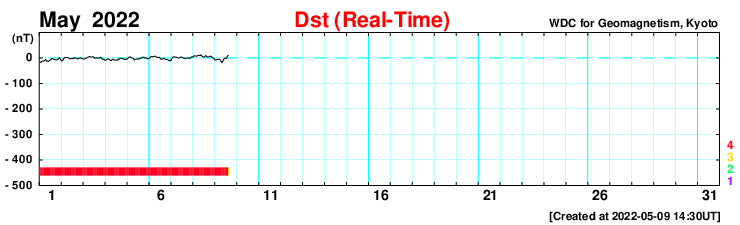
\includegraphics[width=14cm]{./figures/figureGeomag_5.png}

                        \end{figure}

                     \begin{figure}[H]
    
                        \centering
   
                             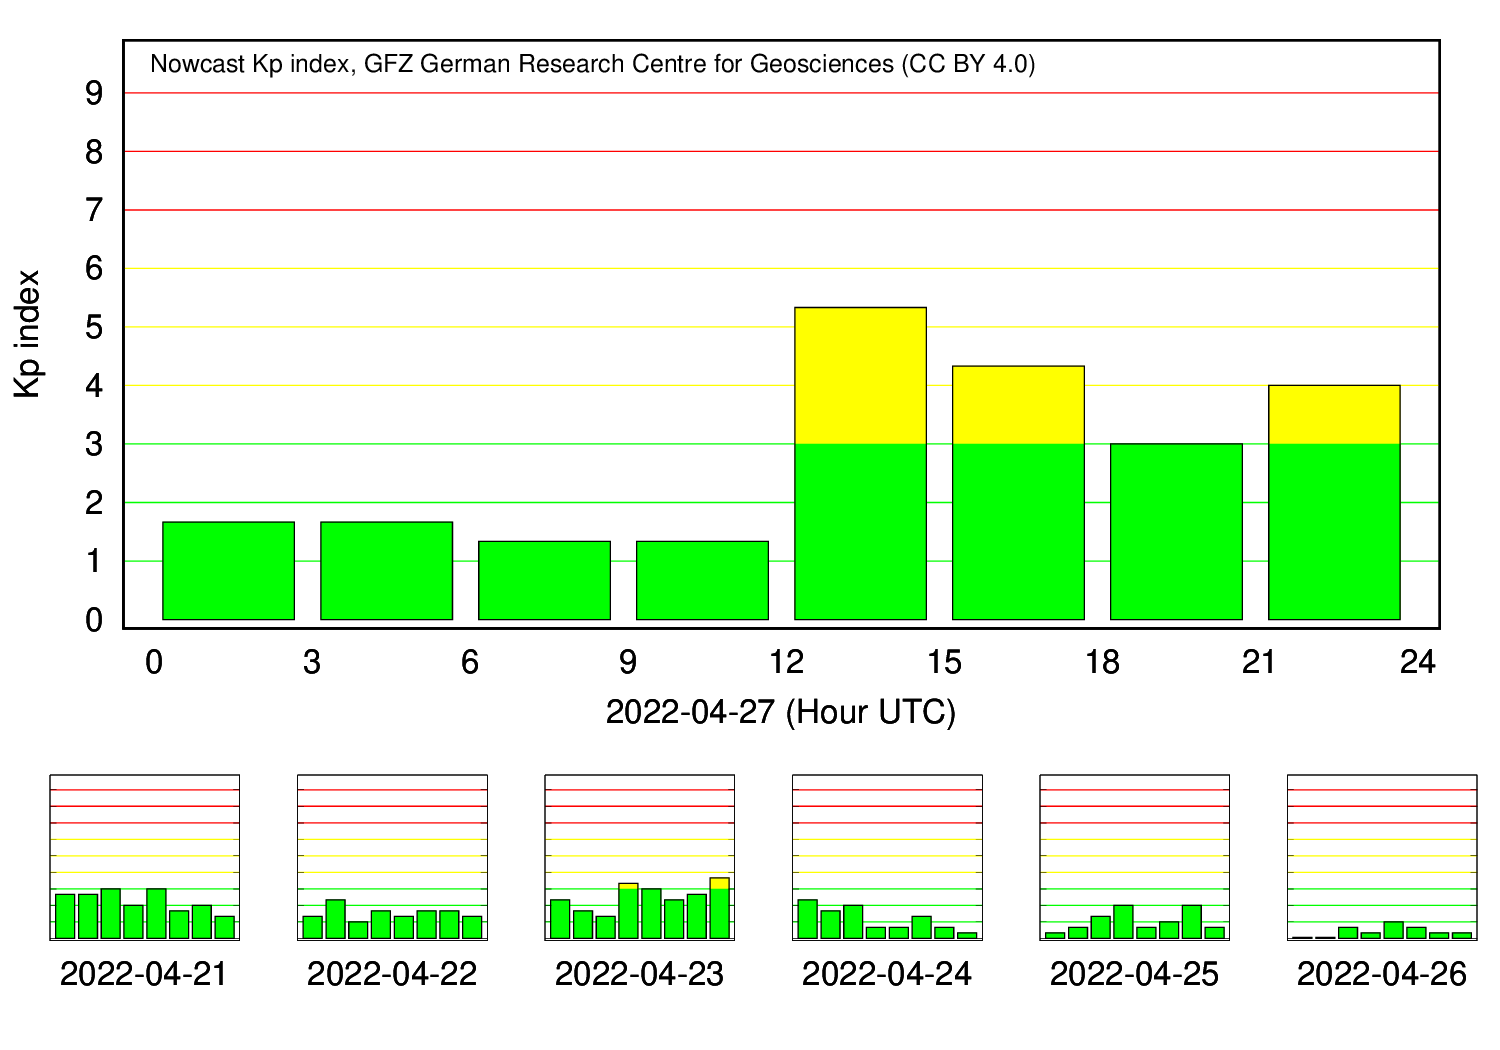
\includegraphics[width=14cm]{./figures/figureGeomag_6.png}

                        \end{figure}

                     \begin{figure}[H]
    
                        \centering
   
                             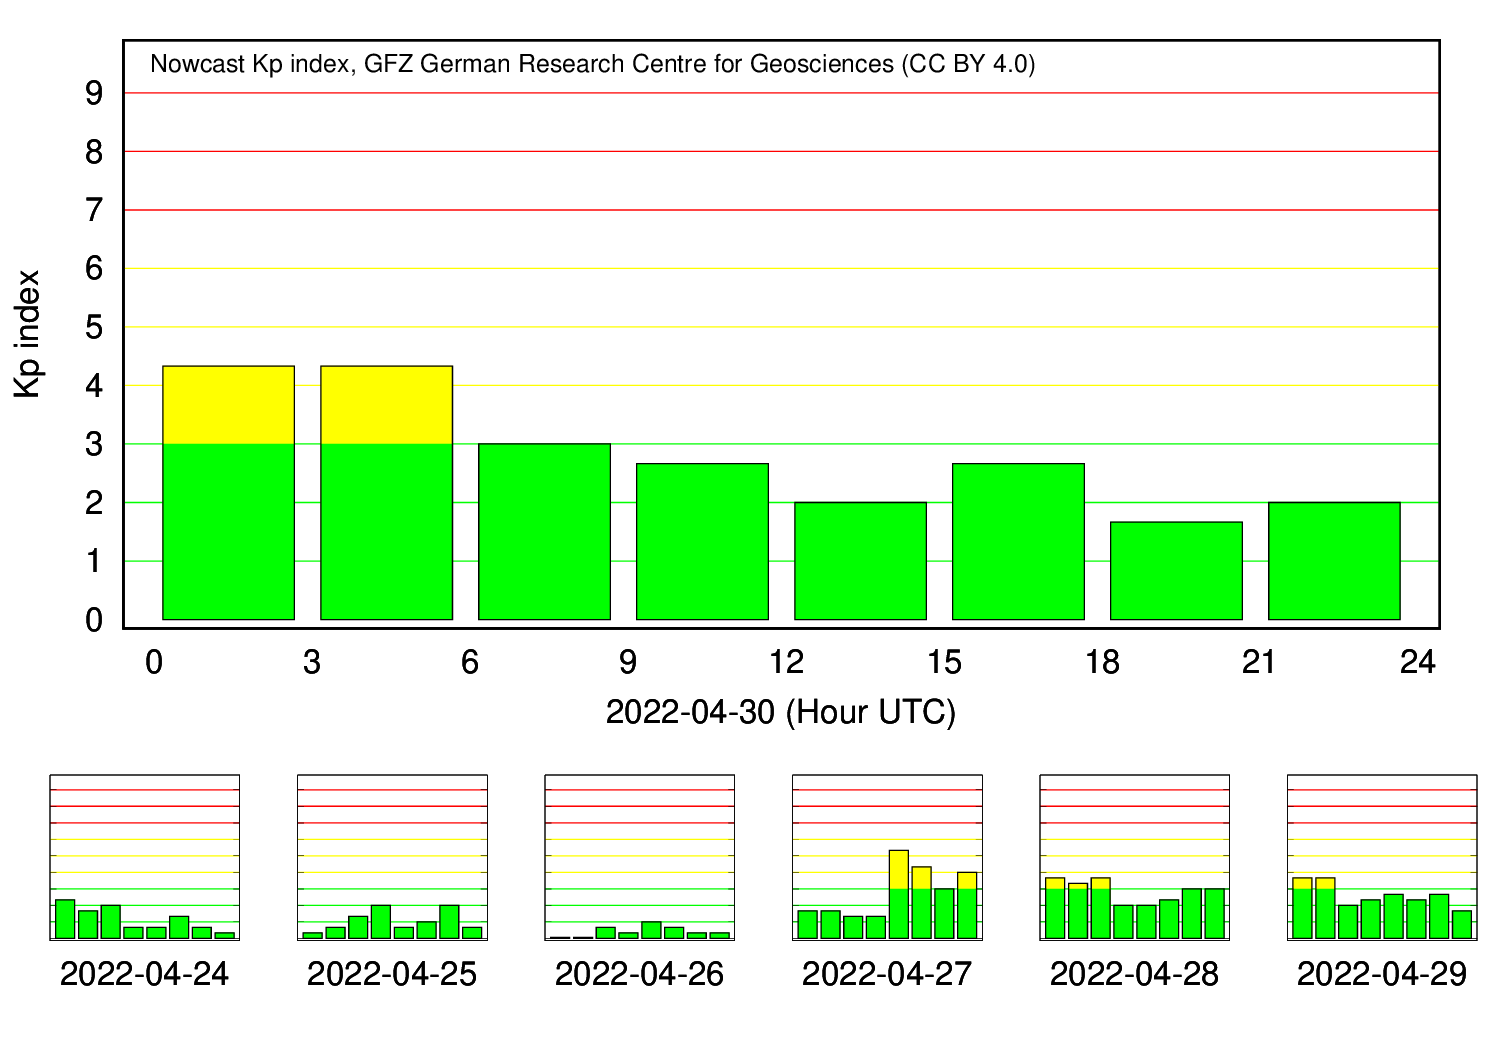
\includegraphics[width=14cm]{./figures/figureGeomag_7.png}

                        \end{figure}

                     \begin{itemize} 
\item Data from the Embrace magnetometer network showed instabilities throughout the period, with some events highlighted:
\item 27th, drop in H component in all seasons, up to -100 nT
\begin{itemize} 
 \item - Geomagnetic activity was more disturbed on 05/24, with the Dst index reaching its minimum value of -30 nT in . Highest Kp of the week was 5+ recorded on 04/27
 \end{itemize} 
\begin{itemize} 
 \item - The auroral activity was intensified in the period from 04/27 to 04/30, highlighting these two days.
 \end{itemize} 
\begin{itemize} 
 \item - Magnetic field measured in the orbit of the GOES satellite showed disturbances on 04/27.
 \end{itemize} 
\end{itemize} 


\end{document}